\subsection{Experimental setup}
Our experimental setup is as follows \cite{versuchsanleitung}:
At first, we measure the peaks of sodium (Na), 
mercury (Hg) and halogen lamps directly with the CCD-spectrometer. 
In case of the Na and Hg lamps, the lamp is installed directly onto 
the underlying construction for the beam path. 
It is then focussed onto the spectroscope by a lense. 
The setup is shown in figure~\ref{fig:const1}.
The halogene lamp is fixed at the end of the beam path, orientated 
in a right angle towrds the spectrometer. The light emmited is 
colliminated by a first lense and re-focussed onto the entrance of 
the spectrometer by a second lense. 
The next step consists of measuring the absorption spectrum 
of iodine. In order to do so, the iodine-pipe is installed 
into the beam path in between of the two lenses, such that 
the light of the halogene lamps passes through as a approximately 
parallel beam. The setup and detail is can be seen in 
figures~\ref{fig:const2} and \ref{fig:const4}.
The pipe is 50 cm long and its diameter is 4 cm. Its inner 
vapour pressure is at 0.5 Torr.

\begin{figure}[!t]
    \begin{captionbeside}[]{
        Photography of the experimental setup when 
        we measure the spectra of the given lightsources. 
        The little white box is the spectroscope.
        }[r]
        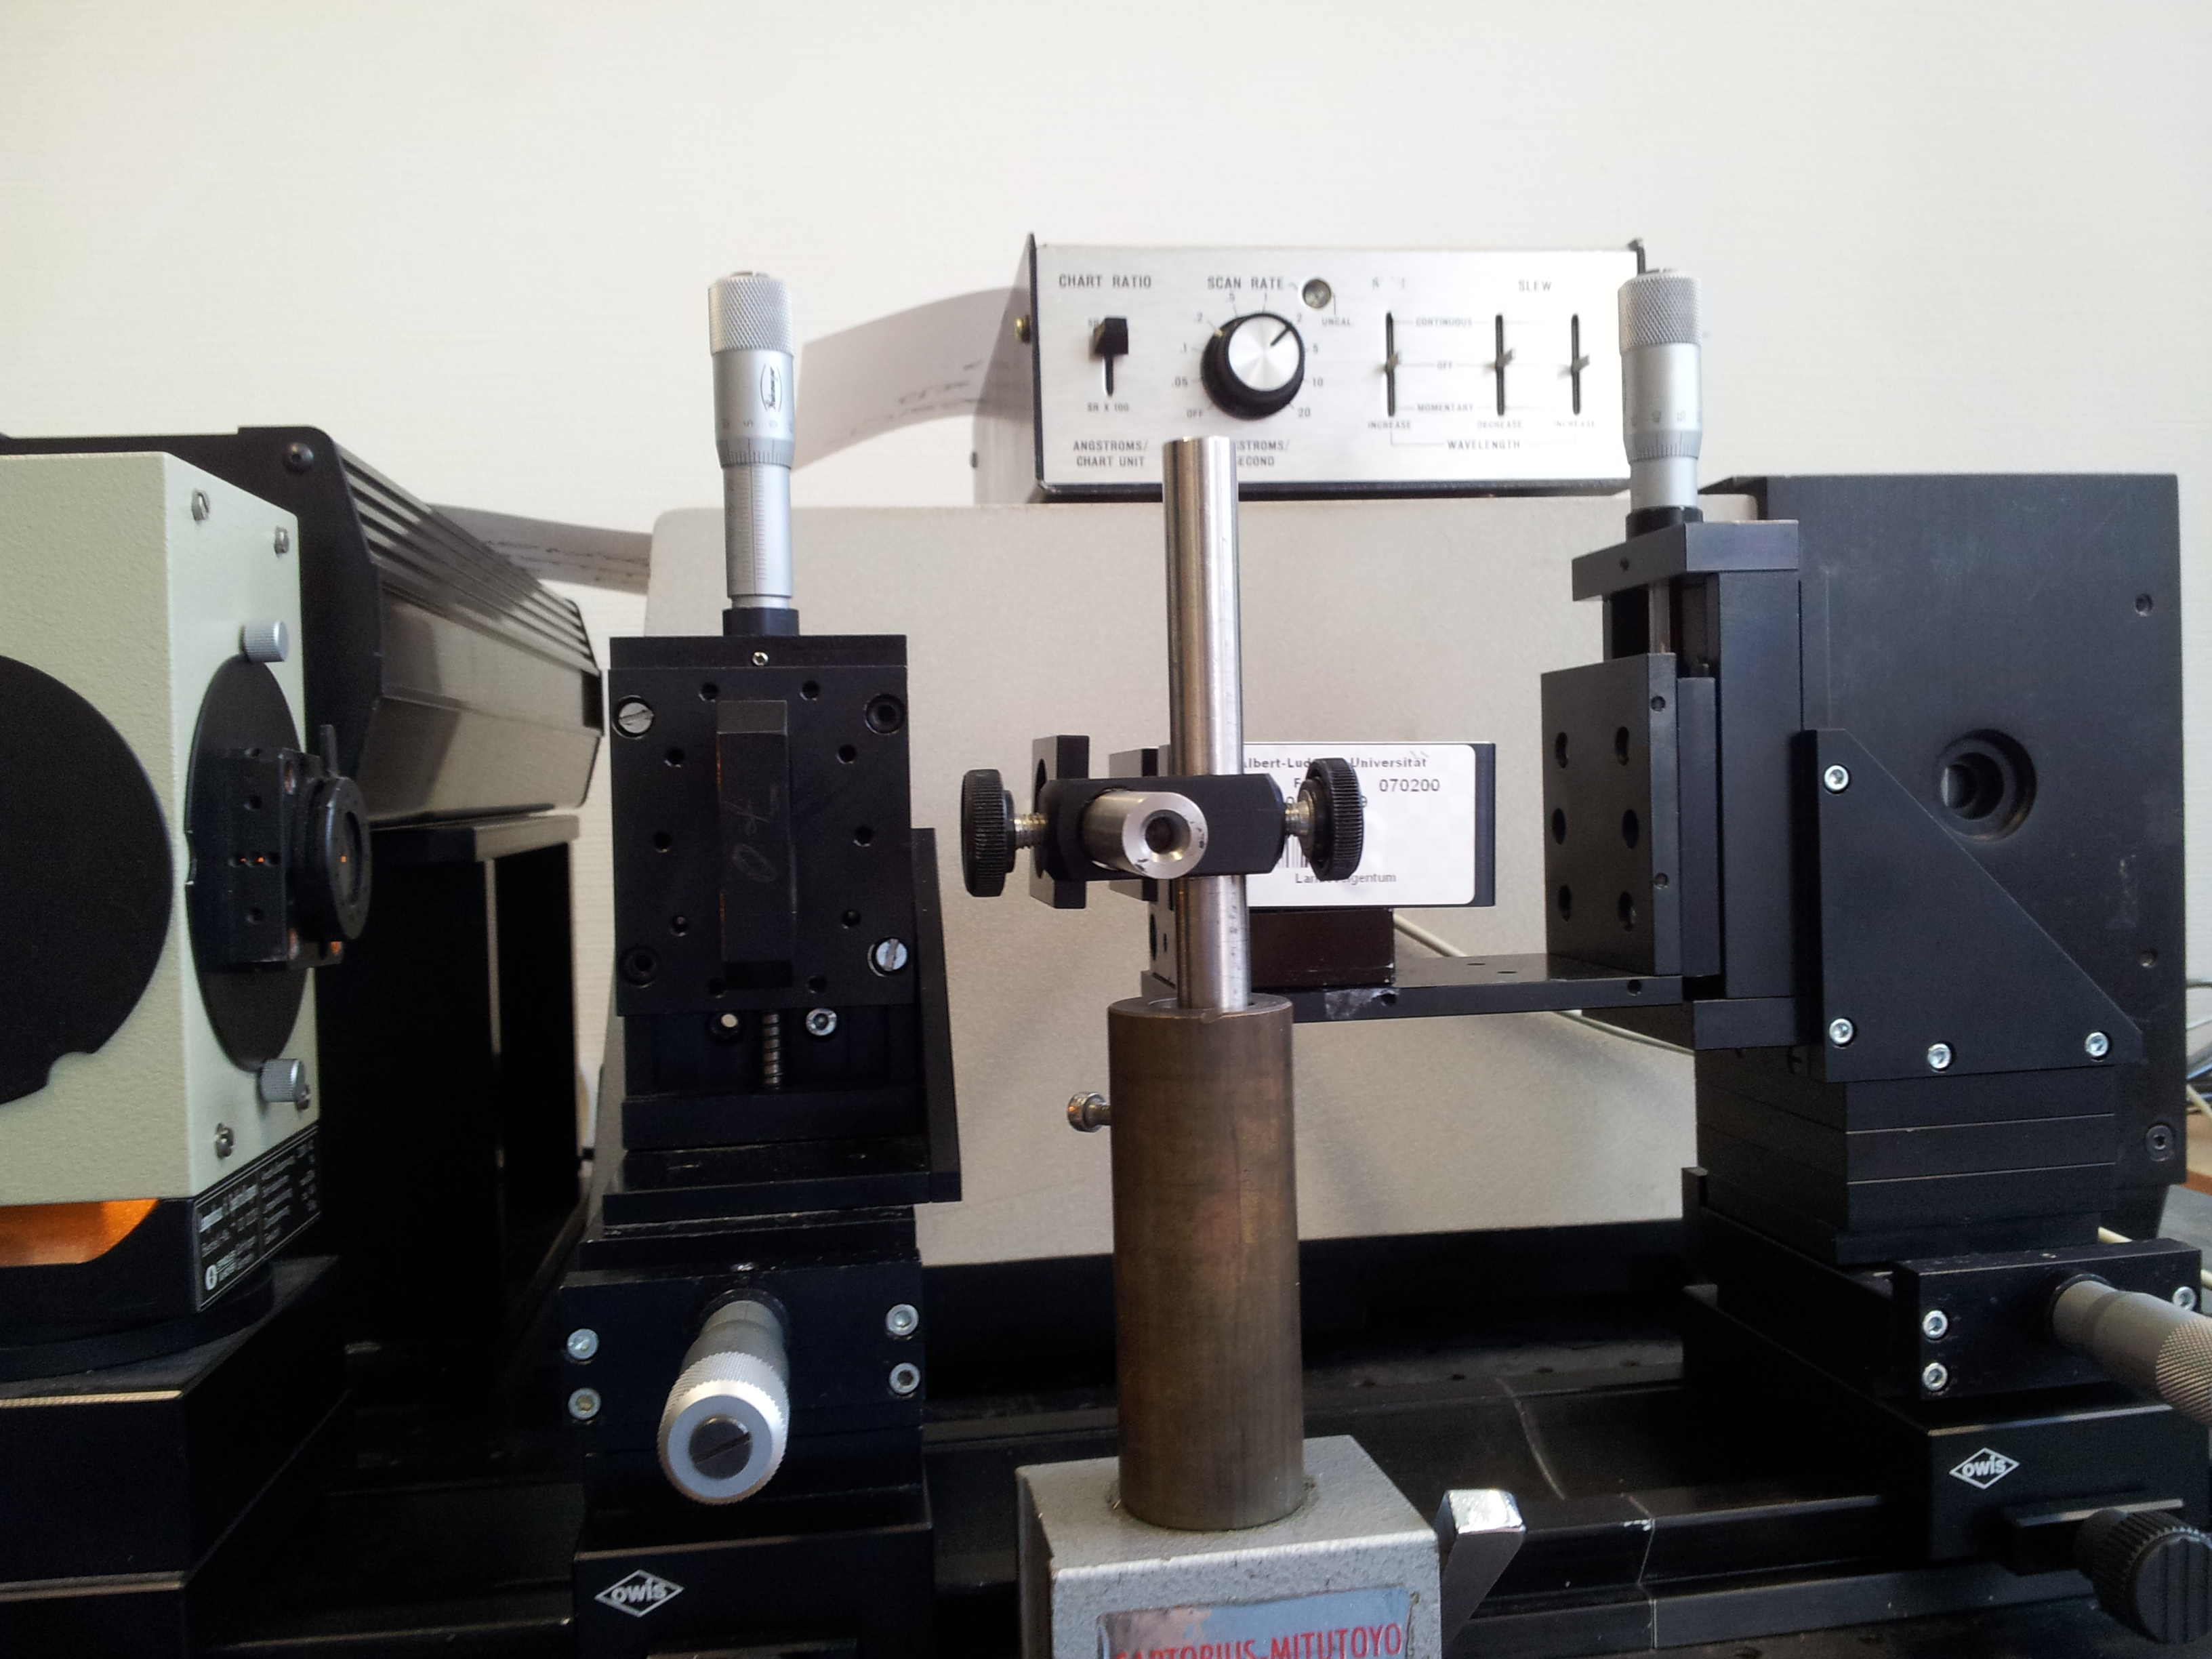
\includegraphics[width=0.48\textwidth]{pics/const1}
    \end{captionbeside}
    \label{fig:const1}
\end{figure}

\begin{figure}[!t]
    \begin{captionbeside}[]{
        Setup with iodinepipe, where the light of the
        halogenlamp will be transmitted through. On the right side
        you can recognize the spectroscope, which will measure
        the absorption lines of the iodine-2 molecules, which
        are located inside of this pipe. It is necessary
        to evacuate them inside of the pipe, because otherwise it
        would sublime in the air.
        }[r]
        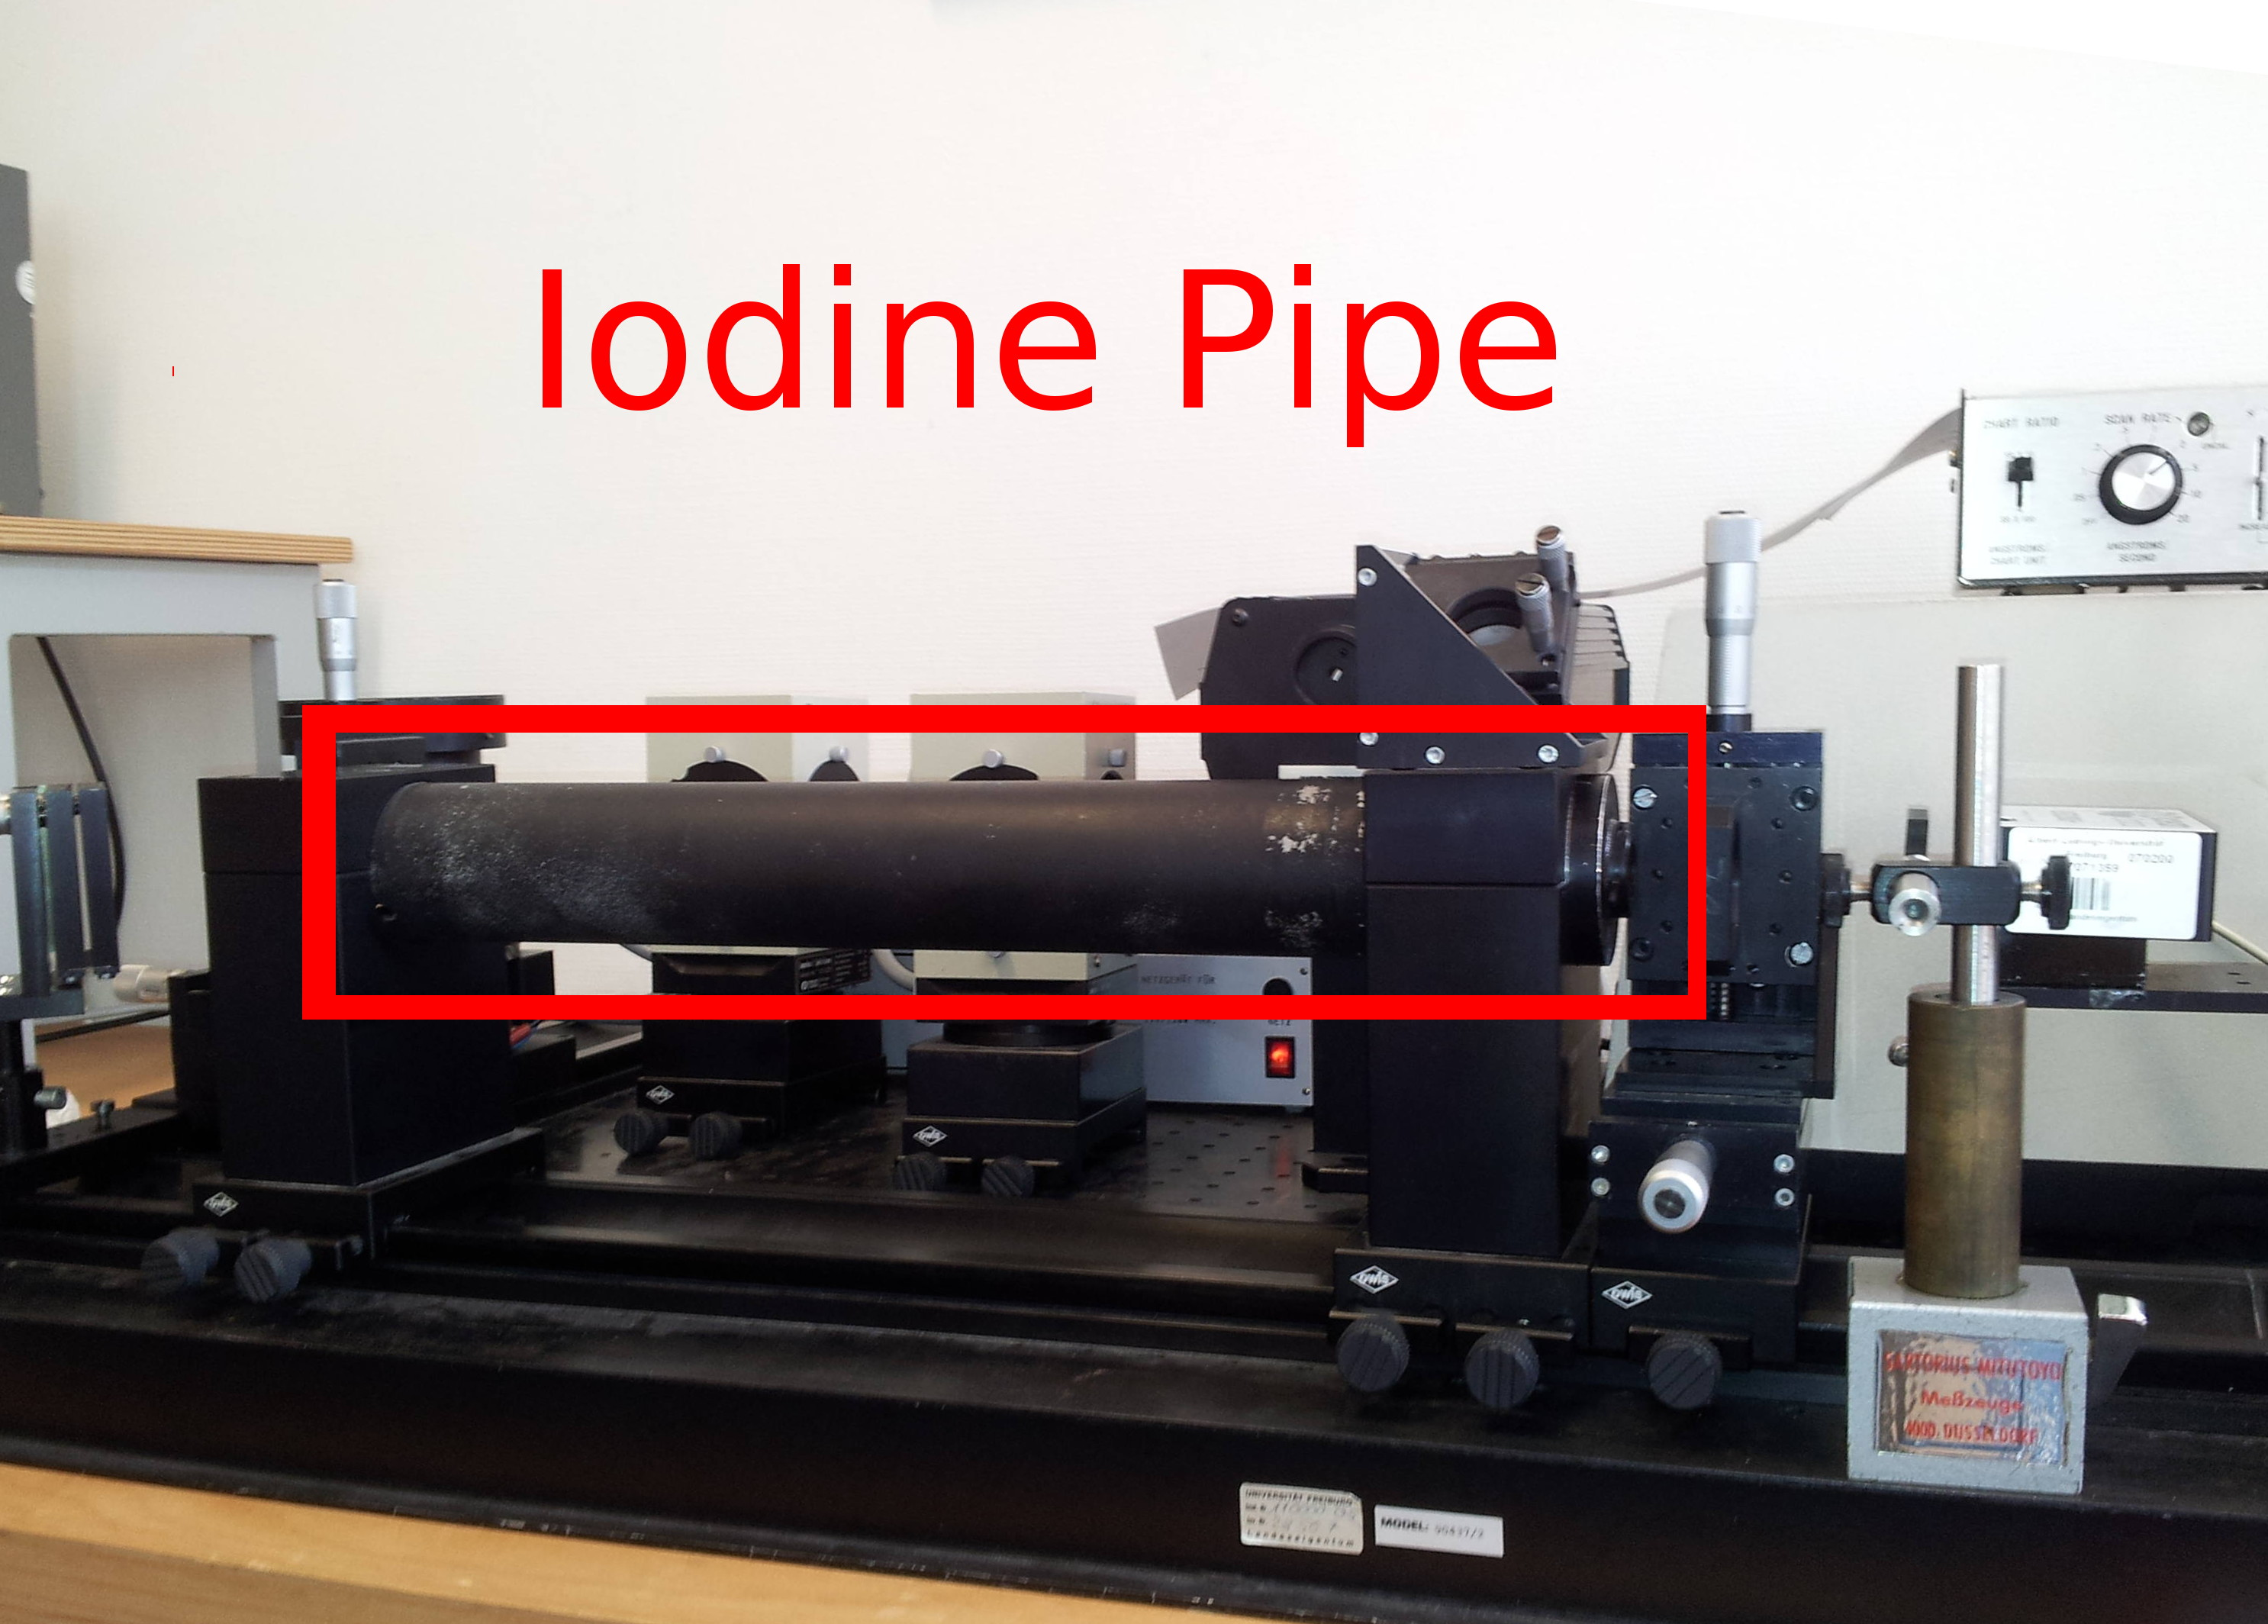
\includegraphics[width=0.48\textwidth]{pics/const2}
    \end{captionbeside}
    \label{fig:const2}
\end{figure}
\begin{figure}[!t]
    \begin{captionbeside}[]{
        Photography of the experiment including the mirrors on
        the left side, the lenses and the opening of the iodinepipe.
        Behind of the lenses there is the lamp whose spectrum will
        be analyzed in the spectroscope, after being transmitted
        through the iodinepipe. 
        }[r]
        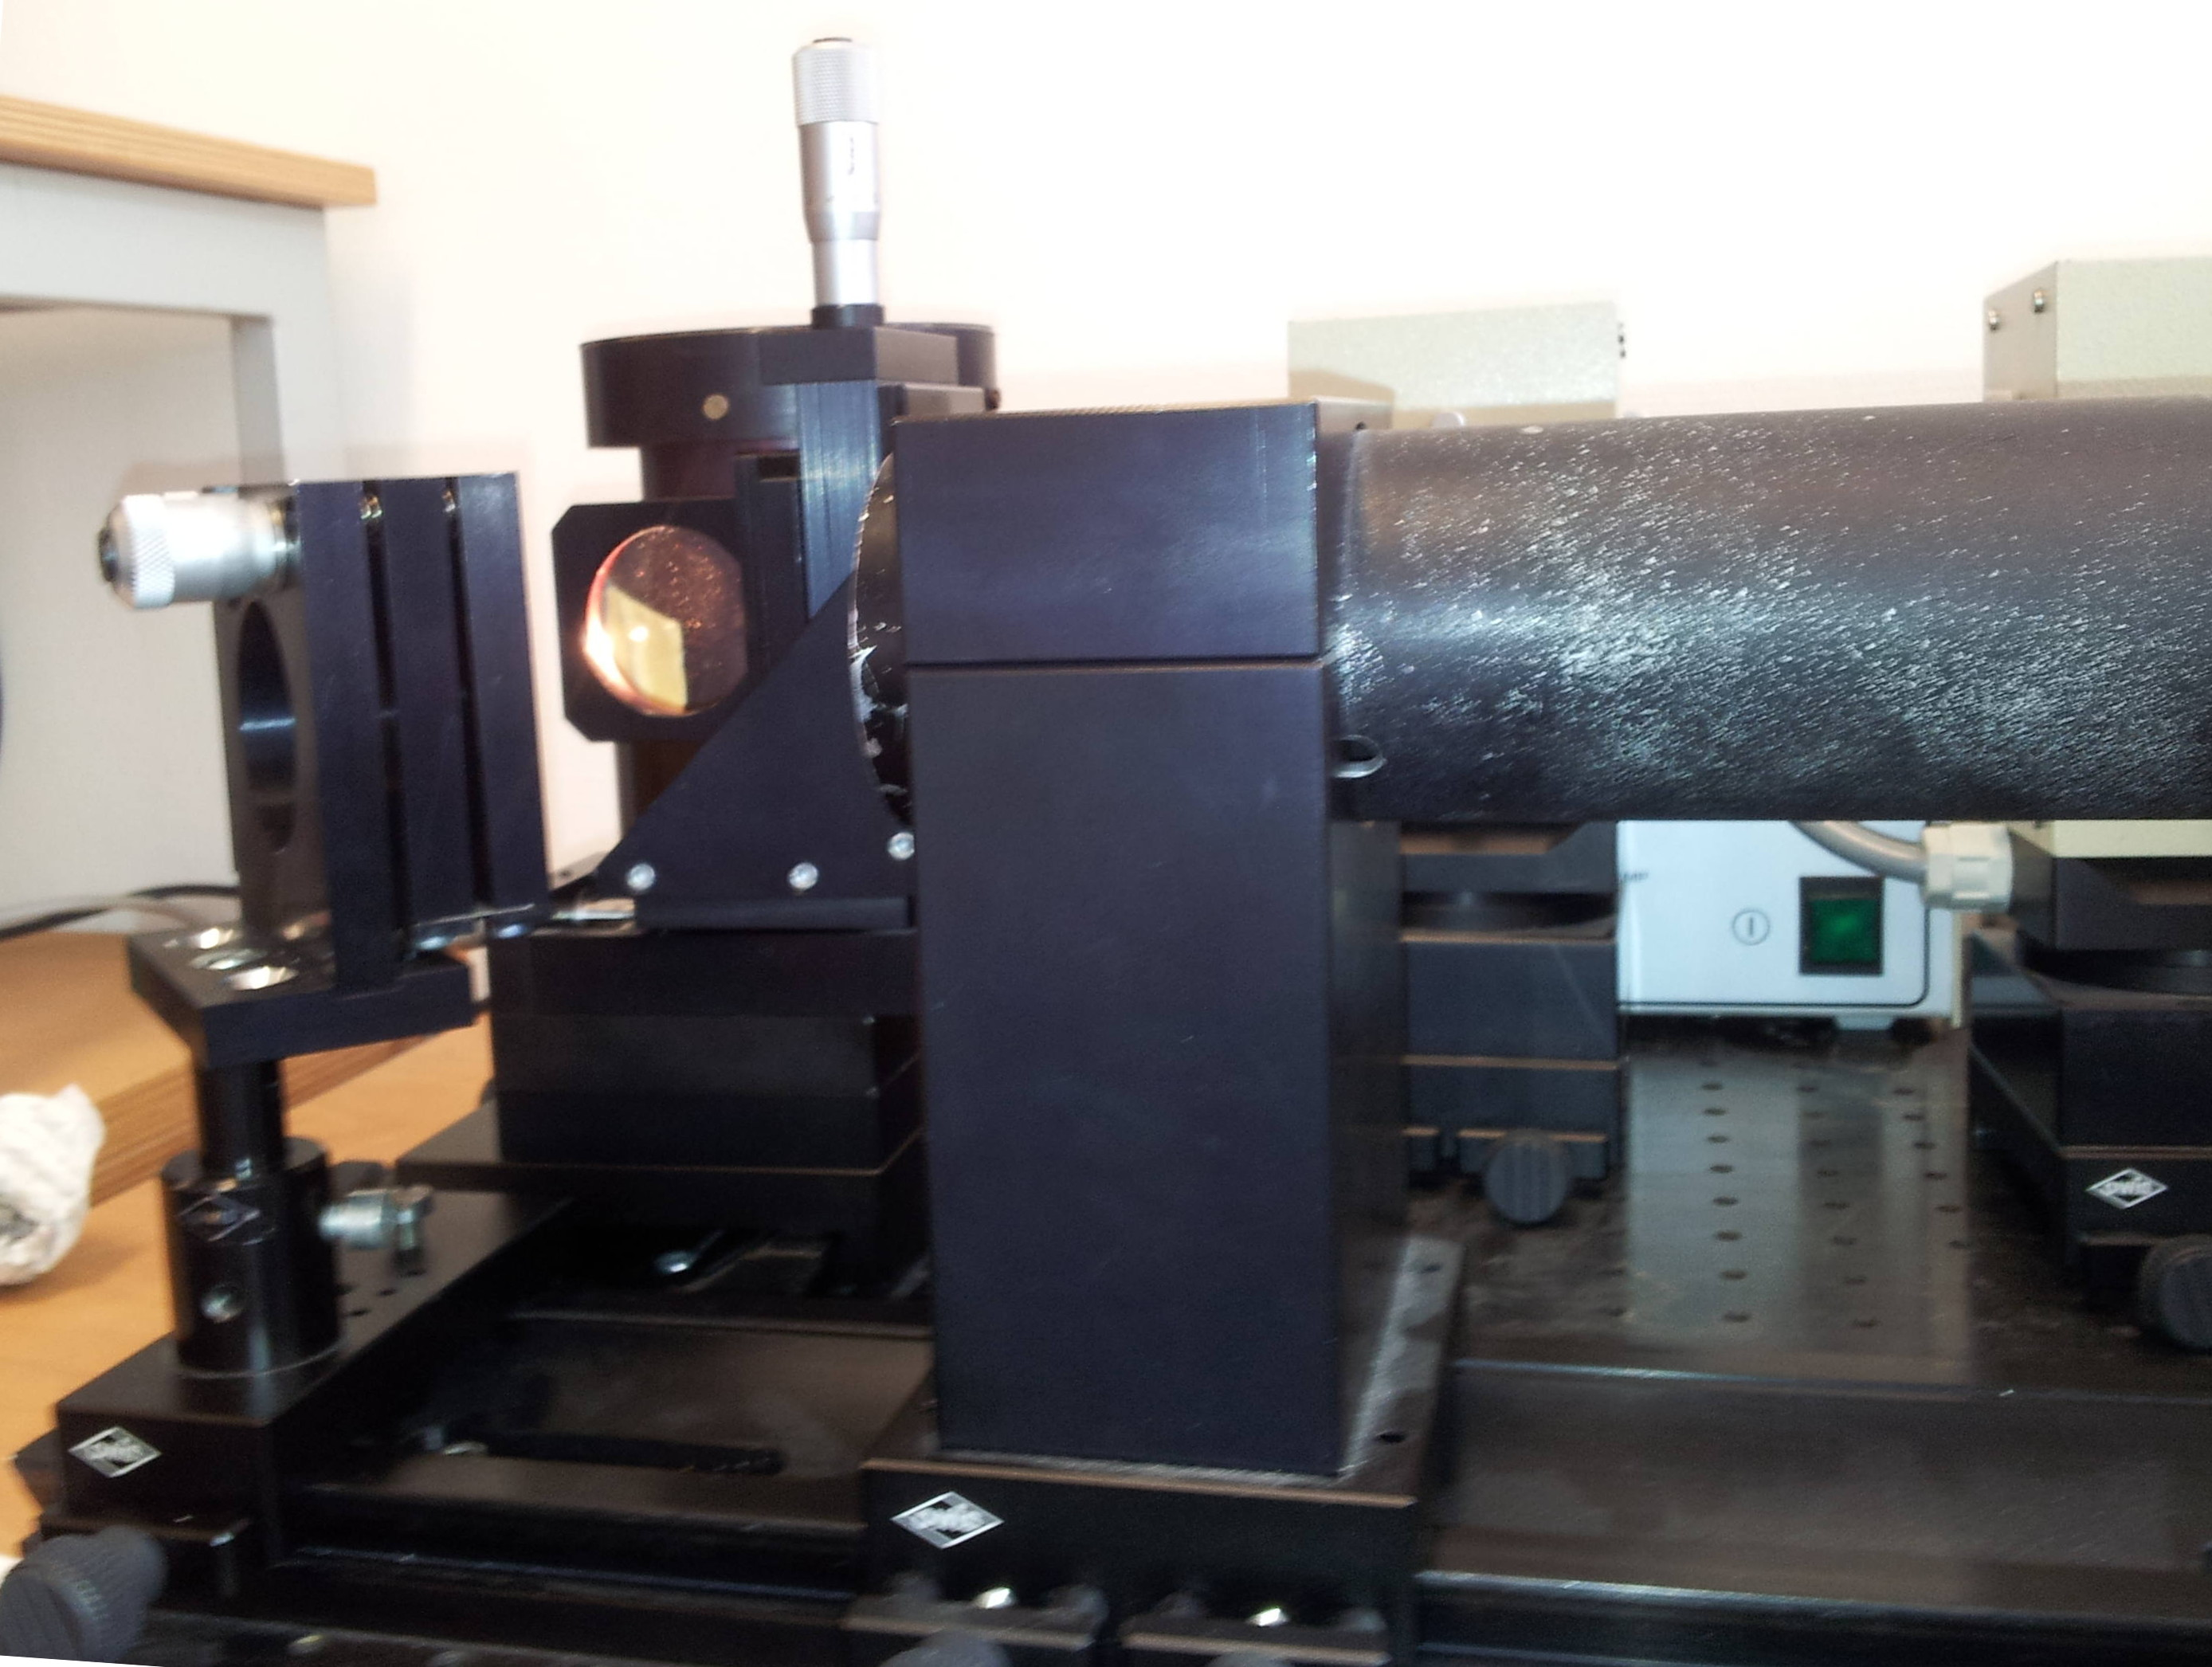
\includegraphics[width=0.47\textwidth]{pics/const4}
    \end{captionbeside}
    \label{fig:const4}
\end{figure}

\subsubsection{CCD-Spectroscope}
The device itself was invented 1969 at the 
\textit{AT\&T Bell Labs}. It is a Charge Couple Device (CCD) using
the photoelectric effect for translating the information of the 
wavelength
of the photon into a potential difference, which can be saved
in terms of condensators. So effectively the number of electrons
resample the number of incoming photons.
It consists of a high sensitivity 2048-element CCD array 
(see table~\ref{tab:ccd} for more details). Each of its sensors 
can roughly be described as a photodiode, meaning a doped
semiconductor with isolaters which in combination is triggered
by photons: If the energy of the photon is higher than the 
band gap of the semiconductor, electrons will be lifted from the
valence band to the conduction band and current-anticurrent pairs
will lead the conducters to save this information. In our case
the incoming light is splitted into its spectral components with
a diffraction grid. For the separated spectral components, the  
CCD-Cells connects position and intensity to measure the 
spectrum in the given window. 
The device used in this experiment is the \textit{USB2000+} 
by the company \textit{ocean optics}
~\cite{versuchsanleitung}. 
The diameter of the opening is $\mu m$ and the spectral range lies 
between 421 to 617 nm with a spectral resolution of 0.6 nm.
The measured spectrum is visualized on the computer, where we
can save it to a file using the software
\textit{SpectraSuite}, which sets the parameters for the 
measurements. There are two possibilites to adjust
the received data from the spectroscope:
\begin{itemize}
    \item Integration time: This manipulates the timespan in 
        which the incoming photons will be counted. It also
        regulates the relative intensity of the signal
        visible in the program, either
        if the required signal was too intense or weak.
    \item Mean value over a number of signals: We can adjust
        whether we want to average the incoming signal due to
        a flickering or noise and over how many incoming signals
        should be averaged.
\end{itemize}


\begin{table}[h]
\centering
\begin{tabular}{| l | l |}
    \hline
    Dimensions & 89.1 mm x 63.3 mm x 34.4 mm \\ 
    \hline
    Detector & Sony ILX511B (2048-element \\
             & linear silicon CCD array) \\  
    \hline
    Range & 200-1100 nm \\ 
    \hline
    Pixels: & 2048 pixels \\ 
    \hline
    Pixelsize & 14 µm x 200 µm \\ 
    \hline
    Optical resolution: & 0.3-10.0 nm \\ 
    \hline
\end{tabular}
    \caption{Specifications of the  CCD Camera \textit{usb2000+}
        \cite{usb2000_site}.}
\label{tab:ccd}
\end{table}

\subsubsection{Spectra of light sources}
In this experiment we will use the nearly continuos spectrum of
the halogenlamp, but before we will calibrate the spectroscope
with the spectra of the other lamps as following.
Since we have very precise values for the emissionspectra of 
the given lightsources \cite{nist} we now immedeatly if
there is a shift in wavelengths (These values for will be given
in the evualation of our results when we compare them with our
results).


